\newpage
\section{Validation: 1D Cartesian}

This section covers the validation of the 1D model developed over the course of
this project. Validation was carried out against analytically tractable cases as
well as with full electromagnetic field simulations in OSIRIS. Several results
from literature were also reproduced as part of this process.

\subsection{Linear Regime}

    As mentioned previously in this document, the linear regime refers to the 
    limit $a_0^2 \ll 1$. Because $a_0^2$ is directly proportional to
    the laser intensity, 

    \subsubsection{Derivation}

    The linear wakefield driven by a laser pulse can be derived from the cold
    fluid equations for an unmagnetized plasma. In three dimensions, the 
    continuity equation is
    \begin{equation*}
        \frac{\partial n_e}{\partial t} + \nabla \cdot (n_e\mathbf{v}_e) = 0,
    \end{equation*}

    the fluid equation is
    \begin{equation*}
        m_e\left[\frac{\partial \mathbf{v}_e}{\partial t} + (\mathbf{v}_e \cdot
        \nabla)\mathbf{v}_e\right] = -e\mathbf{E} - \frac{m_ec^2}{2}\nabla a^2,
    \end{equation*}

    and Poisson's equation is
    \begin{equation*}
        \epsilon_0 \nabla \cdot \mathbf{E} = \epsilon_0\frac{\partial 
        \mathbf{E}}{\partial \mathbf{x}} = e(n_i - n_e),
    \end{equation*}


    where $a = eA/mc^2$ is the normalized vector potential and the 
    $-(mc^2/2)\nabla a^2$ term is the three-dimensional ponderomotive force in 
    the linear limit ($a^2 \ll 1$).
    \vspace{1em}

    To linearize these equations, we treat the amplitude of oscillation as
    small, so the terms containing products of perturbation quantities can be
    neglected. Writing $n_e = n_0 + n_1$, 
    $\mathbf{v}_e = \mathbf{v}_1$, and $\mathbf{E} = \mathbf{E}_1$,
    where quantities with a ``0'' subscript denote the unperturbed equilibrium 
    and quantities with a ``1'' subscript denote small perturbations. Assuming
    a uniform neutral plasma at rest, $\nabla n_0 = \mathbf{v}_0 = 
    \mathbf{E}_0 = 0$, and dropping all second-order terms, the continuity
    equation becomes
    \begin{equation*}
        \frac{\partial n_1}{\partial t} + n_0\nabla\cdot\mathbf{v}_1 = 0,
    \end{equation*}
    the momentum equation becomes
    \begin{equation*}
        \frac{\partial \mathbf{v}_1}{\partial t} = 
        -\frac{e}{m}\mathbf{E}_1 - \frac{c^2}{2}\nabla a^2,
    \end{equation*}
    and Poisson's equation becomes
    \begin{equation*}
        \epsilon_0\nabla\cdot\mathbf{E}_1 = -en_1.
    \end{equation*}

    \begin{note}
    In Poisson's equation, we note that $n_{i0} = n_{e0}$ in 
    equilibrium and assume that $n_{i1} = 0$ (immobile ions).
    \end{note}
    \vspace{1em}

    Taking the partial derivative (with respect to time) of the continuity 
    equation and substituting the momentum and Poisson equations gives the 
    driven plasma oscillation equation:
    \begin{equation}
        \frac{\partial^2 n_1}{\partial t^2} + \omega_p^2 n_1 = 
        \frac{n_0 c^2}{2}\nabla^2 a^2,
        \label{eq:driven_osc}
    \end{equation}

    where $\omega_p^2 = n_0 e^2 / m \epsilon_0 $. Moving to the 
    co-moving frame $\zeta = z - ct$ and using Poisson's equation to relate 
    $n_1$ to $E_z$, equation~\eqref{eq:driven_osc} becomes the driven wave 
    equation for the axial electric field:
    \begin{equation}
        \frac{\partial^2 E_z}{\partial\zeta^2} + k_p^2 E_z = 
        -\frac{k_p}{2}\frac{\partial a^2}{\partial\zeta},
        \label{eq:driven_wake}
    \end{equation} 

    where $k_p = \omega_p/c$. Note that fields are normalized to $E_0 = m_e\omega_p c/e$,
    lengths to $k_p^{-1}$, and times to $\omega_p^{-1}$.~\eqref{eq:driven_wake} is a driven harmonic oscillator in $\zeta$ with the laser intensity gradient 
    $\partial a^2/\partial\zeta$ as the source term. Behind the pulse 
    where $a^2 = 0$, only the homogeneous solution remains, with 
    amplitude and phase set by matching boundary conditions at the back of the 
    pulse.
    \vspace{1em}

    For a circularly polarized sine-squared pulse of the form
    \begin{equation}
        a^2(\zeta) = a_0^2\sin^2\!\left(\frac{\pi\zeta}{L}\right), 
        \quad \zeta_{\rm back} \leq \zeta \leq \zeta_{\rm back} + L,
        \label{eq:sine_pulse}
    \end{equation}
    with a pulse length of $L = \lambda_p = 2\pi/k_p$ (one full plasma 
    wavelength), the wake behind the pulse is
    \begin{align}
        \frac{E_z}{E_0} &= -\frac{\pi}{4}a_0^2\cos\!\left[k_p
        (\zeta - \zeta_{\rm back})\right], 
        \label{eq:Ez_linear} \\
        \frac{\delta n}{n_0} &= -\frac{\pi}{4}a_0^2\sin\!\left[k_p
        (\zeta - \zeta_{\rm back})\right],
        \label{eq:dn_linear}
    \end{align}
    for $\zeta < \zeta_{\rm back}$, and zero ahead of the pulse, where the 
    phase reference $\zeta_{\rm back}$ is the position of the 
    back of the pulse.


    \subsubsection{Sine Pulse: Setup and Parameters}
   
    For this test, a linear wake was driven by a sine-squared pulse
    profile matching the form of~\eqref{eq:sine_pulse}, with 
    $a_0 = 0.25$ placing the simulation in the linear regime 
    ($a_0^2 = 0.0625 \ll 1$).
    \vspace{1em}

    The photon profile was initialized using a \texttt{math\_func} expression:
    \begin{equation*}
        a^2(\zeta) = 0.0625\sin^2\!\left(\frac{\zeta - \zeta_{\rm back}}{2}\right),
        \quad \zeta_{\rm back} \leq \zeta \leq 0,
    \end{equation*}

    with $\zeta_{\rm back} = -2\pi \approx -6.283$ and the pulse
    centered such that its back is at $\zeta_{\rm back}$ and its front at
    $\zeta = 0$.
    \vspace{1em}
    
    The full simulation deck, including grid resolution, time step, and boundary
    conditions, can be found (LINK HERE).

    \subsubsection{Sine Pulse: Results and Comparison}

    The simulated results were plotted against their analytic 
    counterparts,~\eqref{eq:Ez_linear} and~\eqref{eq:dn_linear}. The Python
    function used to plot the analytic expressions is given below. 

    \begin{pythoncode}
    def linear_wake_analytic(zeta, a0, k_p, zeta_pulse_end):
        # Create arrays with the same shape as zeta, filled with zeros
        Ez_E0 = np.zeros_like(zeta)
        dn_n0 = np.zeros_like(zeta)

        # Specifies the z values BEHIND the laser pulse
        behind = zeta < zeta_pulse_end

        # Ez/E0 and dn/n0 should match the analytic expression BEHIND the
        # laser pulse (so, after it's already passed through, this is what the
        # wake should look like)
        Ez_E0[behind] = -(np.pi/4) * a0**2 * np.cos(k_p * (zeta[behind] - zeta_pulse_end))
        dn_n0[behind] = -(np.pi/4) * a0**2 * np.sin(k_p * (zeta[behind] - zeta_pulse_end))

        # Return the analytic result
        return Ez_E0, dn_n0
    \end{pythoncode}

    The position of the back of the laser pulse, $\zeta_{\rm pulse\,end}$, was
    identified numerically at each dump as the location where the simulated
    field amplitude first exceeds a small threshold, accounting for the pulse's
    drift in the simulation window frame. The raw density data was smoothed with
    15 passes of a binomial filter to suppress noise prior to comparing the
    results; the electric field required no such smoothing.
    \vspace{1em}

    Figure~\ref{fig:linear_1D_sine} shows the analytic wake solutions and the 
    corresponding OSIRIS photon kinetic module results at two dump times, dump
    3 (Fig.~\ref{fig:linear_1D_dump3}) and dump 50 (Fig.~\ref{fig:linear_1D_dump50}).
    In each panel, the top plot shows the axial electric field $E_z / E_0$ 
    and the bottom plot shows the density perturbation $\delta n / n_0$. 

    \begin{note}
        The abrupt cutoff of the analytic curves reflects the fact that the 
        wake, by construction, should only exist behind the pulse. So, ahead
        of the position of the back of the pulse ($\zeta_{\rm back}$), the
        analytic solution is exactly zero.
    \end{note}

    \begin{figure}[htbp]
    \centering
    \begin{subfigure}{0.48\textwidth}
        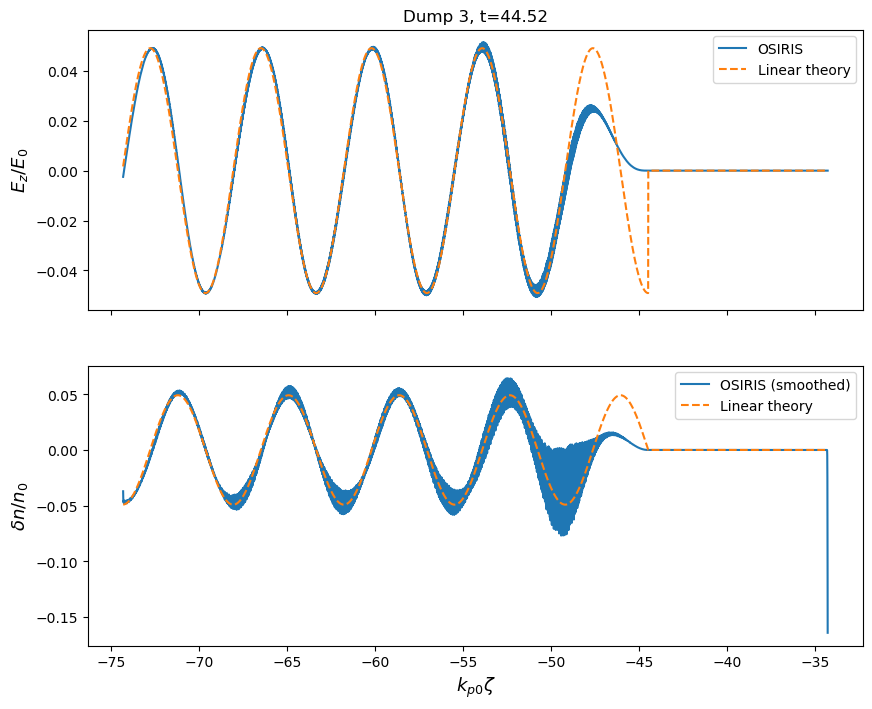
\includegraphics[width=\linewidth]{figures/validation-1D/dump3-linear.png}
        \caption{Dump 3}
        \label{fig:linear_1D_dump3}
    \end{subfigure}
    \hfill
    \begin{subfigure}{0.48\textwidth}
        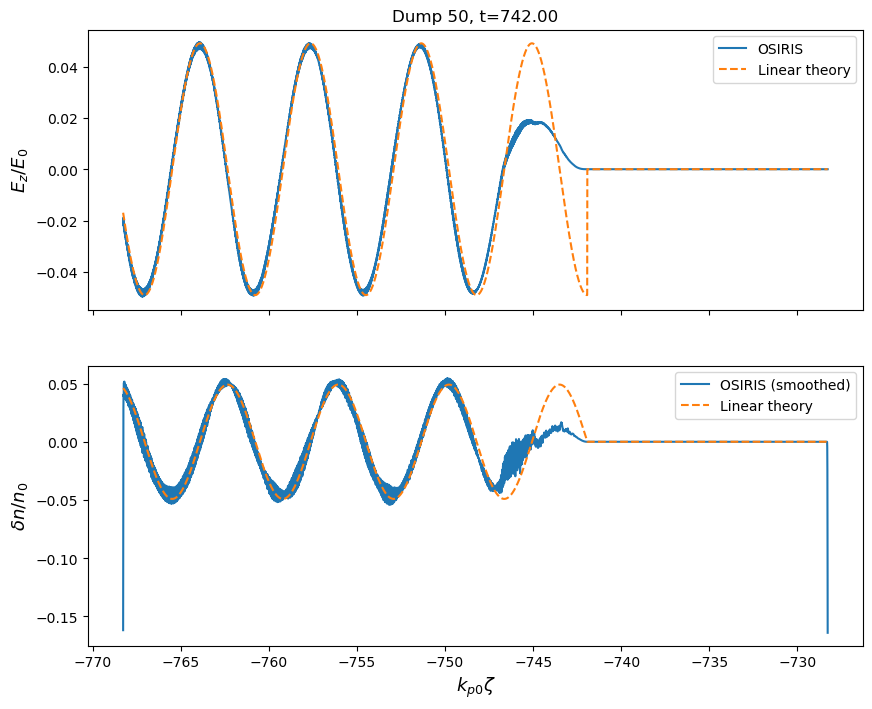
\includegraphics[width=\linewidth]{figures/validation-1D/dump50-linear.png}
        \caption{Dump 50}
        \label{fig:linear_1D_dump50}
    \end{subfigure}
    \caption{Comparison of simulated (OSIRIS) and analytic linear wake 
    solutions for a sine-squared pulse at two different dump times.
    Top: axial electric field $E_z/E_0$. Bottom: density perturbation
    $\delta n/n_0$.}
    \label{fig:linear_1D_sine}
    \end{figure}

    \subsubsection{Notes}

\subsection{Nonlinear Regime}
    
    Unlike the linear regime, the nonlinear regime doesn't ...

    \subsubsection{Derivation}

    Following Esarey et al. (2009), the 1D nonlinear wake potential
    $\phi$ satisfies
    \begin{equation}
        k_p^{-2}\frac{\partial^2\phi}{\partial\xi^2} = 
        \frac{1+a^2}{2(1+\phi)^2} - \frac{1}{2},
        \label{eq:nonlinear_wake}
    \end{equation}
    where $\gamma_\perp^2 = 1+a^2$ is the transverse quiver Lorentz factor
    of the plasma electrons. Unlike the linear case, this equation cannot
    be solved analytically in closed form for a general pulse profile, so
    it is instead integrated numerically as an initial value problem,
    starting from undisturbed plasma ahead of the pulse.


    For this regime, rather than analytically (mathematically) solving for
    the expressions of the wake, etc., we will just write a simple solver, 
    which we can test by trying to replicate the figure from the (BLANK) paper.

    \subsubsection{Solver Implementation}

    \begin{pythoncode}
    def solve_nonlinear_wake(a0, L_rms, k_p, k_pulse, zeta_range):

        # The analytic expression of the Gaussian profile we're using for the
        # photon distribution
        def a2(z):
            return a0**2 * np.exp(-z**2 / (2*L_rms**2)) * np.cos(k_pulse*z)**2

        # Make the second-order differential equation into a system of first
        # order differential equations
        def rhs(z, y):
            phi, dphi = y
            numerator = 1 + a2(z)
            d2phi = k_p**2 * (numerator / (2*(1+phi)**2) - 0.5)
            return [dphi, d2phi]

        # Initial conditions: phi = dphi/dzeta = 0 ahead of the pulse, where the
        # plasma is undisturbed
        y0 = [0.0, 0.0]

        # Evaluation grid for the returned solution
        zeta_eval = np.linspace(zeta_range[0], zeta_range[1], 10000)

        # Set a maximum step size so the fast oscillations can be resolved
        # (the cosine term in the above equation for a^2)
        max_step = (2*np.pi/k_pulse) / 20.0

        # Solve the system given all of this information
        sol = solve_ivp(rhs, [zeta_range[0], zeta_range[1]], y0, t_eval=zeta_eval, method='RK45', rtol=1e-8, atol=1e-10, max_step=max_step)

        zeta_sol = sol.t
        phi = sol.y[0]
        dphi = sol.y[1]
        numerator = 1 + a2(zeta_sol)

        # Ez/E0 = -dphi/dzeta (normalized axial field from the potential).
        Ez_E0 = -dphi

        # Nonlinear density perturbation
        n_n0 = (numerator + (1+phi)**2) / (2*(1+phi)**2)
        dn_n0 = n_n0 - 1.0

        return zeta_sol, Ez_E0, dn_n0, phi
    \end{pythoncode}

    Using this, we can replicate Figure 8 in the Esarey paper:
    
    \subsubsection{Gaussian Pulse : Setup}

        

    \subsubsection{Gaussian Pulse : Results}


    \subsubsection{Gaussian Pulse : Setup}


    \subsubsection{Gaussian Pulse : Results}




  \subsection{Comparison with Full EM Simulation}
    \subsubsection{zpulse Equivalent Setup}
    \subsubsection{Wake Amplitude Comparison}
    \subsubsection{Photon Phase Space Comparison}
  \subsection{Reproduction of Trines et al. 2007}
    \subsubsection{Parameters and Setup}
    \subsubsection{Results: Figure 2 Comparison}
    \subsubsection{Discussion and Discrepancies}
